\ProvidesFile{ap-graphics.tex}[2021-08-23 graphics appendix]

\begin{VerbatimOut}{z.out}
\chapter{GRAPHICS}

There are many ways to make graphics for \LaTeX.
I like to use a system that uses \LaTeX\ fonts
so the appearance of the output is more professional.
\end{VerbatimOut}

\MyIO


\begin{VerbatimOut}{z.out}


\section{\LaTeX\ \TikZLogo\ package}
\index{TikZ@\TikZLogo}  
\end{VerbatimOut}

\MyIO


\begin{VerbatimOut}{z.out}


\subsection{Yin and yang}

This Yin and yang example was done by Thomas G. Kristensen \cite{kristensen}.
This is the ``traditional Taijitu symbol from Chinese philosophy''.\\
\ix{Kristensen, Thomas G.//Taijitu symbol//Yin and yang symbol}

\index{TikZ@\TikZLogo}  

\begin{tikzpicture}
  % Yin and yang
  % Author: Thomas G. Kristensen
  
  % color one half of a unit circle                                              
  \begin{scope}
    \clip (0,0) circle (1cm);
    \fill[black] (0cm,1cm) rectangle (-1cm, -1cm);
  \end{scope}

  % fill heads                                                                   
  \fill[black] (0,0.5) circle (0.5cm);
  \fill[white] (0,-0.5) circle (0.5cm);

  % fill eyes                                                                    
  \fill[white] (0,0.5) circle (0.1cm);
  \fill[black] (0,-0.5) circle (0.1cm);

  % outer line                                                                   
  \draw (0,0) circle (1cm);

\end{tikzpicture}
\end{VerbatimOut}

\MyIO



\begin{VerbatimOut}{z.out}

\section{Mathematica (which uses Wolfram Language)}
\ix{Mathematica}
\end{VerbatimOut}

\MyIO


\begin{VerbatimOut}{z.out}

\section{MATLAB}
\ix{MATLAB}
\end{VerbatimOut}

\MyIO


\begin{VerbatimOut}{z.out}

\section{\protect\METAPOSTLogo\ (uses \LaTeX\ fonts)}
\index{METAPOST@\METAPOSTLogo}  

I did these \METAPOSTLogo\ \cite{metapost} examples
for Yanghyun Kim \cite{kim2009}.
\ix{Kim, Yanghyun}
\end{VerbatimOut}

\MyIO


\begin{VerbatimOut}{z.out}

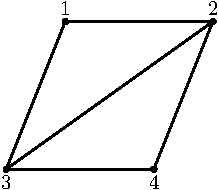
\includegraphics{gr-kim1.pdf}
\todoerror{need source code}  

\vspace{0.1truein}

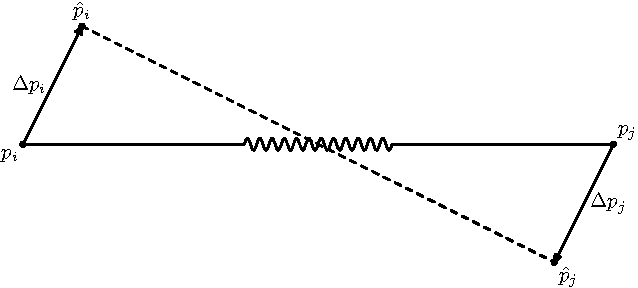
\includegraphics{gr-kim2.pdf}
\todoerror{need source code}  
\end{VerbatimOut}

\MyIO


\begin{VerbatimOut}{z.out}

\subsection{\METAPOSTLogo\ Tally Example}
\label{ss:tally-example}

Whenever I use files with numbers in them I like to put leading zeros
in the names so they will be listed in order in the directory.

These 20 graphics (gr-tally-01.pdf through gr-tally-20.pdf)

\vspace*{6pt}

{%
  % Let * represent zero or more spaces!
  % Method 1: \def\g#1{ requires using \g*{10} for 10.
  %           Two shifted characters, { and } are needed.
  % Method 2: \def\g#1/{ requires using \g*10/ for 10.
  %           One unshifted character, / is needed.
  \def\g#1/{\includegraphics[scale=0.5]{gr-tally-#1.pdf}}%

  % Note that tabular* instead of tabular is used below.
  %   The {\textwidth} makes the total width of the table the width
  % of the printed area of the page.
  %   The @{\kern2\parindent} puts blank space the width of two
  % paragraph indents before the first column.
  %   The @{extracolsep{\fill}} adds \fill space between all subsequent
  % columns.
  %   The lll left justifies the next three columns.
  % after the column.
  %   The @{\kern2\parindent} puts blank space the width of two
  % paragraph indents before the first column.
  \begin{tabular*}{\textwidth}{@{\kern2\parindent}@{\extracolsep{\fill}}lll@{\kern2\parindent}}%
    \g 01/& \g 02/& \g 03/\\
    \g 04/& \g 05/& \g 06/\\
    \g 07/& \g 08/& \g 09/\\
    \g 10/& \g 11/& \g 12/\\
    \g 13/& \g 14/& \g 15/\\
    \g 16/& \g 17/& \g 18/\\
    \g 19/& \g 20/\\
  \end{tabular*}%
}
\noindent were produced by

\MyI{misc/tally.mp}

\end{VerbatimOut}

\MyIO


\begin{VerbatimOut}{z.out}

\section{R}
\ix{R}
\end{VerbatimOut}

\MyIO


\begin{VerbatimOut}{z.out}

\section{\TikZLogo\ and PGF (uses \LaTeX\ fonts)}
\index{TikZ@\TikZLogo}
\ix{PGF}
\end{VerbatimOut}

\MyIO


\begin{VerbatimOut}{z.out}

\subsection{Clock}
\end{VerbatimOut}

\MyIO


\begin{VerbatimOut}{z.out}

The idea for this clock was originally
from a Google+ posting by
Afamefuna ``Ferdy'' Ibeabuchia.  \ix{Ibeabuchia, Afamefuna ``Ferdy''//PGF}
\index{TikZ@\TikZLogo}

\hbox to\textwidth{%
  \hfil
  \begin{tikzpicture}
    \def\CenterRadius{0.04cm}
    \def\InnerTickRadius{3.6cm}
    \def\OuterTickRadius{3.8cm}
    % Make \LR be an abbreviation for \LabelRadius so the
    % lines below will fit within the width of the page.
    \def\LabelRadius{4.5cm}      \let\LR=\LabelRadius
    \def\HourHandRadius{2.5cm}   \def\HourHandBase{0.3cm}
    \def\MinuteHandRadius{3cm}   \def\MinuteHandBase{0.4cm}
    \def\SecondHandRadius{3.5cm} \def\SecondHandBase{0.5cm}
    \def\DS{\displaystyle}
    \fill (0,0) circle (\CenterRadius);
    \foreach \i in {0,30,...,330}
    \draw (\i:\InnerTickRadius)--(\i:\OuterTickRadius);
    \node at (  0:\LR) {$\DS \qquad \sqrt9 + 9 - 9$};        %  3
    \node at ( 30:\LR) {$\DS \frac{9+9}9$};                  %  2
    \node at ( 60:\LR) {$\DS \frac{\sqrt9\sqrt9}9$};         %  1
    \node at ( 90:\LR) {$\DS 9 + \frac9{\sqrt9}$};           % 12
    \node at (120:\LR) {$\DS \frac{99}9$};                   % 11
    \node at (150:\LR) {$\DS 9 + \frac99$};                  % 10
    \node at (180:\LR) {$\DS \sqrt[\scriptstyle 9]{9^9}$};   %  9
    \node at (210:\LR) {$\DS 9 - \frac99$};                  %  8
    \node at (240:\LR) {$\DS 9 - \sqrt9 + \lceil.9\rceil$};  %  7
    \node at (270:\LR) {$\DS 9 - \frac9{\sqrt9}$};           %  6
    \node at (300:\LR) {$\DS \sqrt9\,! - \frac99$};          %  5
    \node at (330:\LR) {$\DS \sqrt9 + \frac99$};             %  4
    % In the following
    %   ABBREVIATION    DESCRIPTION
    %   deg             degrees
    %   min             minutes
    %   sec             seconds
    % for second hand:
    %   (9 sec/60 sec) * 360 deg = 54 deg;
    %   90 deg - 54 deg = 36 deg
    \draw[rotate around={36:(0,0)}]
      (-\SecondHandBase,\SecondHandBase) -- (\SecondHandRadius,0)
        -- (-\SecondHandBase,-\SecondHandBase) -- cycle;
    % for minute hand:
    %   (9 min/60 min) * 360 deg = 54 deg;
    %   90 deg - 54 deg = 36 deg
   \draw[rotate around={36:(0,0)}]
     (-\MinuteHandBase,\MinuteHandBase) -- (\MinuteHandRadius,0)
       -- (-\MinuteHandBase,-\MinuteHandBase) -- cycle;
    % for hour hand:
    %   (9 min * (60 sec/1 min)) + 9 sec) / 3600 sec
    %     = 549 sec / 3600 sec = 0.1525
    %   The hour hand is 0.1525 of the way from 9:00 to 10:00.
    %   Each hour is 30 degrees on the clock, so the hour hand
    %   position is
    %     30 deg * 0.1525 = 4.575 deg past 9:00
    %   180 deg - 4.575 deg = 175.425 deg
    \draw[rotate around={175.425:(0,0)}]
      (-\HourHandBase,\HourHandBase) -- (\HourHandRadius,0)
      -- (-\HourHandBase,-\HourHandBase) -- cycle;
  \end{tikzpicture}
  \hfil
}
\end{VerbatimOut}

\MyIO


\begin{VerbatimOut}{z.out}

\subsection{Glider}
\ix{Hirzel, Alex//Glider emblem representing the hacker community}

The glider
is a pattern from the Game of Life,
and it's used as an emblem representing the hacker community.

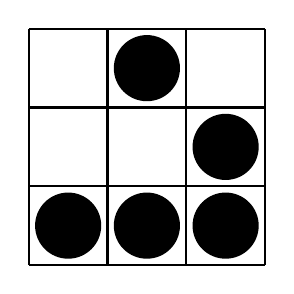
\begin{tikzpicture}[thick]
  \draw (0,0) grid (3,3);
  \foreach \c in {(0,0), (1,0), (2,0), (2,1), (1,2)}
    \fill \c + (0.5,0.5) circle (0.42);
\end{tikzpicture}
\end{VerbatimOut}

\MyIO
